% !TEX root = ../thesis.tex

\section{Discussion}

We present a data-driven social signal prediction framework, which allows us to investigate the dynamics and correlations among interpersonal social signals. We first formalize the social signal prediction framework, and describe several subtasks with different inputs and outputs. To build the models, we leverage our Haggling dataset collected from hundreds of participants, by using the sensing and measurement techniques presented in this thesis. In particular, the various nonverbal channels in the Haggling dataset provides a crucial opportunity to computationally study their dynamics. We demonstrate clear evidence that the social signals emerging in genuine interactions are predictive each other, by presenting frameworks, predicting speaking and predicting social formations.

We believe the approach described in this chapter is an important direction to endow machines with the nonverbal communication ability. However, there are several unexplored directions in this chapter, and two important questions are discussed in this section. 

\subsection{Predicting More Complicated Signals}
We may tackle predicting more complicated social signals using the social signal prediction framework presented in this chapter. For example, we predict body gestures of the target individual by using communication partners' body signals as input:

\begin{gather}	
\mathbf{B}^0 (t_0:t) = \mathcal{F}_{(B1,B2)\rightarrow B0} \left( \mathbf{B}^1 (t_0:t), \mathbf{B}^2 (t_0:t) \right) .
\end{gather}

We have tested this approach by implementing a neural network. For the implementation, we follow the work of \cite{holden2016deep} to first learn a human motion manifold space, and then build another neural network to find the mapping between the input signals (body motions from other individuals) and the output body motion (the target individual's body motion). We found that this approach produces human-like body motions with dynamic movements on legs and upper bodies, but it was less clear that this approach can capture the social behaviors showing a strong correlation across interacting individuals. Two core reasons can be considered about the limited performance: (1) the quantity of our dataset is not sufficient to model the correlation among high dimensional signal spaces, and (2) the metric used for training models as loss function and also for the evaluation metric, the Euclidean (or L2) distance, may not be ideal to effectively extract the subtle correlations among high dimensional social signals.

\subsection{Evaluating Social Signal Prediction}
The output of social signal prediction should satisfy the following two requirements: (1) the predicted signals should be within a feasible human motion space showing realistic human motions, and (2) the predicted signals should follow the social rules, responding to the behaviors of communication partners. However, it is challenging to evaluate these requirements, because there is no objective metric to quantify ``realistic'' or ``social'' properties in behaviors. Notably, the L2 distance between the predicted signals and ground-truth may not be a good metric because it also does not consider such properties. For example, although several human behaviors can be still acceptable given the same input in our social signal prediction task, this metric penalizes them if they are different from the single ground-truth motion, regardless their quality. Due to the reason, the L2 metric often favors the output close to the mean of the data distribution, although it is qualitatively far from the expected output. The similar issue has been discussed in human motion forecasting field~\cite{mnih2012conditional, Fragkiadaki_2015_ICCV, jain2016structural, zhou2018autoconditioned}. In body gesture prediction trial described above, we found a similar issue as shown in the Table~\ref{table:predBody_errors}, where the mean pose of the training set outperforms our prediction result, although the mean pose is is far from the realistic motion with only a static pose, while our result shows human-like motion with reasonable dynamics. This issue also causes the social signal modeling more challenging.

%We found that the L2 distance is reliable for the signals in relatively lower dimensions, showing that the lower error clearly means the better quality.

\begin{table}[t]
	\centering
	%	\footnotesize
	%\caption{Social Body Gesture Prediction Errors}
	\begin{tabular}{c| c| c}
		
		\hline
		%Types & Avg. dist. (cm) & Std.(cm) & Min dist. (cm)  & Max dist. (cm)\\
		Types & Avg. Joint Errors (cm) & Std.\\
		\hline
		%Mirroring buyer & 11.60 &2.70\\
		%\hline
		%		Mirroring input seller & 10.86 &2.49\\
		%		\hline
		Mean Pose & \underline {\textbf{7.83}} & 2.33\\
		\hline
		Prediction by our method & 8.72 & 2.00\\
		\hline
	\end{tabular}
	\caption{Social Body Gesture Prediction Errors (cm). The error is computed by averaging L2 distance of all joints using the Ground Truth body motion. \label{table:predBody_errors}}
\end{table}

\subsection{Modeling More Diverse Social Interaction}
In this chapter, we demonstrate social signal modeling in a triadic scene, focusing on the Haggling scenario we defined. As an important future direction, more general social scenarios (e.g., polyadic interaction among an arbitrary number of individuals) needs to be considered. This direction requires a way to build a larger social interaction database in more diverse social scenarios, which may not be handled by our studio setup. The video sequence capturing social interaction, millions of which are already available on the Internet, can be an important source for this direction, although obtaining 3D signals from these in-the-wild monocular videos is a challenging problem. In our recent work, we show a promising result in this direction by presenting a monocular total capture method~\cite{Xiang2019}. How to model social interaction among an arbitrary number of communication partners is another issue, since our current approach assumes a fixed number of communication partners. 
%Triadic is chosen and studied? What about other cases?

%
%\subsection{Necessity of High Resolutional Social Signals}  
%Do we need all this measurment? My own belief?
%
%\subsection{Considering More General Interaction}    o
%Triadic is chosen and studied? What about other cases?


%
%We present a data-driven social signal prediction task, which allows us to investigate the dynamics and correlations among interpersonal social signals. We first formalize the social signal prediction framework, and describe several subtasks with different inputs and outputs. To build the models, we leverage our Haggling dataset. In particular, the various nonverbal channels in the Haggling dataset provides a crucial opportunity to computationally study their dynamics. We demonstrate a clear evidence that the social signals emerging in genuine interactions are predictive each other. Notably, how to evaluate the performance of the predicted output is a big challenge, and we present an indirect method to check the speaking status of the predicted body motion. This method enables us to quantify the motion prediction quality, considering the required social rules the output needs to follow. 
%
%We believe the approach described in this chapter is an important direction to endow machines with the nonverbal communication ability. As the first step, we focus on a triadic social scenario, but, to consider more general social situations, a way to collect more diverse 3D social signal data in various scenes should be considered. As a direction, collecting the 3D social signals in-the-wild videos can be a way (e.g., \cite{Xiang2019}), although measuring 3D signals from a monocular video is still a challenging problem.
%%We hypothesize that data is the key to understanding nonverbal communication. We hope the direction of this thesis, showing the new approaches in sensing, measuring, and modeling social signals, can inspire research community to advance this field more actively. 
%
%\subsection{Why About Predicting More Complicated Signals?}
%
%\subsection{Evaluating Social Signal Prediction}
%
%\subsection{Predicting Body Gestures}
%\label{section:pred_body}
%Predicting body motion in social situations by using other subjects' signals is challenging, because the correlation between body signals are subtle and less explicit. To study this, we present three baseline approaches here. 
%
%\paragraph{By Using Predicted Social Formation.} The first approach uses only the social formation information of other subjects:
%\begin{gather}	
%\mathbf{J}^0(t_0:t) = \mathcal{F}_{P12\rightarrow J} \left( \mathbf{X}_p^1(t_0:t), \mathbf{X}_p^2(t_0:t) \right).
%\end{gather}
%This is an ill-posed problem with diverse possible solutions, because the formation signals of communication partners barely tell us about the detailed behavior of our target person. Yet, we can consider several required properties of the predicted skeleton. For example, the body location and orientation need to satisfy the social formation property, and when the target person's location is changing the appropriate leg motion needs to be predicted. Intuitively, we expect the predicted skeleton shows a similar social amount of information, location and orientations, as in social formation prediction, but using more complicated structure, body motion. In that sense, we can divide the function $\mathcal{F}_{P12\rightarrow J}$ into two stages: predicting a social formation by $\mathcal{F}_p$ described in Eq.~\ref{eq:pred_formation} and predicting 3D body motion from the predicted social trajectory $\mathbf{Y}_p (t_0:t)$:
%\begin{gather}	
%\mathbf{J}^0 (t_0:t) = \mathcal{F}_{P0\rightarrow J} \left(   \mathcal{F}_p \left( \mathbf{X}_p^1(t_0:t), \mathbf{X}_p^2(t_0:t) \right) \right) \nonumber \\ 
%= \mathcal{F}_{P0\rightarrow J} \left( \mathbf{Y}_p (t_0:t)  \right),
%\label{eq:pred_p2J}
%\end{gather}
%where $\mathcal{F}_{P0\rightarrow J}$ is a mapping between the target subject's own social trajectory to body skeleton. Since the trajectory (position and orientations) is a sub-part of the body behavior, we expect the predicted skeleton to contain similar signals as the social trajectory. For the function $\mathcal{F}_{P0\rightarrow J}$, we follow a similar approach to the work of Holden et al.~\cite{holden2016deep}. As in the Holden's work, we train an autoencoder to find the motion manifold space. As a major difference, we do not use foot step generator, and directly regress from the trajectory to the motion manifold space. We train this model in our dataset only, since the walking and running motion used in \cite{holden2016deep} is rare in our scenarios. 
%
%\paragraph{By Using Body Motions as Input.} We can use the entire body signals of conversational partners as input for our function:
%\begin{gather}	
%\mathbf{J}^0 (t_0:t) = \mathcal{F}_{J12\rightarrow J} \left( \mathbf{J}^1 (t_0:t), \mathbf{J}^2 (t_0:t) \right) .
%\end{gather}
%In this particular example, we expect ``better" prediction quality than the previous baseline by using other subject's body motions as a cue to determine the target person's body motion. We found that this method shows more diverse upper body motion, responding to the motions of other subjects. To this end, we present a hybrid method combining the upper body prediction results of this method to the root and leg motions of the previous method. The lower part of the output model follows the movement to keep to the social formation and upper body produce more dynamic behaviors responding to input signals.
%
%\paragraph{By Using Body Motions as Input.} We can also use the face motions of conversational partners as input for our function:
%\begin{gather}	
%\mathbf{J}^0 (t_0:t) = \mathcal{F}_{F12\rightarrow J} \left( \mathbf{F}^1 (t_0:t), \mathbf{F}^2 (t_0:t) \right) .
%\end{gather}
%
%The main motivation of this approach is that face motion provides stronger cues to predict the speaking status of the target person (or turn-taking of the interaction). Thus, we expect this approach may provide a better performance in predicting body signals, especially considering the turn-taking timing of the scenes. 
%
%\subsection{Predicting Facial Signals}
%We also predict the facial expression signal of the target person, by taking facial signals of other subjects as input. 
%\begin{gather}	
%\mathbf{F}^0(t_0:t) = \mathcal{F}_{F12\rightarrow F} \left( \mathbf{F}_p^1(t_0:t), \mathbf{F}_p^2(t_0:t) \right).
%\end{gather}
%
%
%
%\begin{table}[t]
%	\centering
%	%	\footnotesize
%	%\caption{Social Body Gesture Prediction Errors}
%	\begin{tabular}{c| c| c}
%		
%		\hline
%		%Types & Avg. dist. (cm) & Std.(cm) & Min dist. (cm)  & Max dist. (cm)\\
%		Types & Avg. Joint Errors (cm) & Std.\\
%		\hline
%		%Mirroring buyer & 11.60 &2.70\\
%		%\hline
%		%		Mirroring input seller & 10.86 &2.49\\
%		%		\hline
%		Mean Pose \underline {\textbf{7.83}} & 2.33\\
%		\hline
%		Traj2Body & 8.31 & 2.26\\
%		\hline
%		% 		body2Body & 8.19 (2.01)\\
%		Body2Body & 8.72 & 2.00\\
%		\hline
%		% 		body2Body & 8.19 (2.01)\\
%		Traj2Body (lower body) + Body2Body (upper body) & 8.61  & 1.84\\
%		\hline
%	\end{tabular}
%	\caption{Social Body Gesture Prediction Errors (cm). Body orientation and face orientation are computed between estimated and GT unit vectors (need to be fixed) \label{table:predBody_errors}}
%\end{table}
%
%
%
%\begin{table}[t]
%	\centering
%	%	\footnotesize
%	\begin{tabular}{l| l}
%		\hline
%		%Types & Avg. dist. (cm) & Std.(cm) & Min dist. (cm)  & Max dist. (cm)\\
%		Input Signal & Accuracy\\
%		\hline
%		\hline
%		Ground-truth Own Body & 79.94 \% \\       %new
%		\hline
%		Ground-truth Other Seller's Body & 75.28 \% \\       %new
%		\hline
%		\hline
%		Mean Pose & 51.03\% \\       %new
%		\hline
%		Traj2Body & 51.42\% \\       %new
%		\hline
%		Body2Body & 52.97\% \\       %new
%		\hline
%		Body2Body+Traj2Body & 52.78\% \\       %new
%		\hline
%		Face2Body & \underline {\textbf{67.68}}\% \\       %new
%		\hline
%		Face2Body+Traj2Body & 66.60\% \\       %new
%		\hline
%	\end{tabular}
%	\caption{We evaluate the speaking status of predicted models to quantitatively measure the quality of them. This table shows speaking status prediction accuracies, where the speaking status is predicted from the synthesized body motions from the specified sources.\label{table:pred_body_error_speaking}}
%\end{table}
%
%
%
%\subsection{Body Gestures Prediction}
%As described in Section~\ref{section:pred_body}, we predict body motion of the target person by three different sources, which we refer to as: traj2body, body2body, and face2body. In the ``traj2body" method, the body motion is directly regressed from the estimated social formation (location and orientation) of the target person. This method shows reasonable leg motions following the trajectory movements, but has minimum upper body motion. Examples are shown in the fourth row of Fig.~\ref{fig:qualitative}. In ``body2body" method, we predict the target person's body motion by using other subjects' body motion as input. This motion does not take into account the global formation cues, but shows more dynamic body motions by responding to other subjects' motion. We can combine both methods, by merging the formation and leg motion from the first method to the upper body motion from the second method. Examples are shown in the fifth row of Fig.~\ref{fig:qualitative}. In the ``face2body" method, we use other seller's face motion as a source to predict the body motion of the target person. Similarly, we can combine this output with the leg motion of ``traj2body" method. The prediction results show human-like social behaviors including location, body and face orientation, leg motion, and hand gestures. 
%
%We first quantitatively evaluate the predicted body gesture using the common L2 distance. We consider a baseline method, ``Mean Pose", by computing the average posture of all training data and constantly use it as prediction output. As shown in Table~\ref{table:predBody_errors}, the L2 error of this baseline shows the best performance, although this motion is not realistic and not suitable for social situations.
%
%For our new metric described in Section~\ref{section:evaluation}, we predict the speaking status from the predicted motions. We use our pre-trained speaking status classifier that takes own body signals as input, which shows about $76\%$ prediction accuracy in Table~\ref{table:speaking_class}. Then, we compute the speaking status accuracy using ground truth speaking status. The speaking is closely related to the turn-taking timing in the interaction, and this method penalizes if the predicted body motion does not follow the speaking timing of the ground truth data. As shown in Table~\ref{table:pred_body_error_speaking}, the baseline method using the mean pose only shows almost a chance level accuracy ($51.03\%$), showing mostly no speaking motions regardless the situations\footnote{The position and orientation part of the input values are still changing, which makes sometimes our classier produces speaking label as output.}. The prediction by ``body2body" method shows a better performance, but still poor in this metric. The prediction by `` face2body" method shows the best performance with a significant margin, since, presumably, the face cue of other subjects provides a strong clue to determine the speaking timing, as demonstrated in Table~\ref{table:speaking_class}. This experiment shows interesting correlations among position, orientation, body, and face signals among interacting groups. %As shown in this result, our social signal prediction method shows a reasonable performance in modeling the dynamics of social signals, and our evaluation method can be used to quantify the output.
%
%%
%%
%%\section{Evaluating Social Signal Prediction}
%%\label{section:evaluation}
%%The output of social signal prediction should satisfy the following two requirements: (1) the predicted signals should be within a feasible human motion space showing realistic human motions, and (2) the predicted signals should follow the social rules, responding to the behaviors of communication partners. However, it is challenging to evaluate these requirements, because there is no objective metric to quantify ``realistic" or ``social" properties in behaviors. Notably, the L2 distance between the predicted signals and ground-truth may not be a good metric because it also does not consider such properties. For example, although several human behaviors can be still acceptable given the same input in our social signal prediction task, this metric penalizes them if they are different from the single ground-truth motion, regardless their quality. Due to the reason, the L2 metric often favors the output close to the mean of the data distribution, although it is qualitatively far from the expected output. The similar issue has been discussed in human motion forecasting field~\cite{mnih2012conditional, Fragkiadaki_2015_ICCV, jain2016structural, zhou2018autoconditioned}. In particular, we found that the first requirement can be satisfied by enforcing the output in the motion manifold space~\cite{holden2016deep}, but there is no good way to enforce the second requirement.
%%
%%
%%In this work, we present a way to quantify the quality of social signal prediction outputs (particularly body motion prediction), focusing on the turn-taking rule in social interaction (particularly for the second requirement). We found that the L2 distance is reliable for the signals in relatively lower dimensions, showing that the lower error clearly means the better quality. Classifying speaking status described in Section~\ref{subsection:ssp_pred_speak} is an example of it.  Our idea is to ``guess" the speaking status of the predicted body motion, and quantify it by using the ground-truth speaking status, as shown in Figure~\ref{fig:evaluation_bySpeakclass}. This method potentially penalizes only the turn-taking rule in the social situation, allowing diverse motion outputs as correct answers. To satisfy the turn-taking rule, the model still needs to learn the social rules by observing the input social signals. To produce speaking status from the predicted body gestures, we use our speaking status classifier described in Section~\ref{subsection:ssp_pred_speak}. This metric is not ideal due to the use of our speaking status classifier which is not perfect, and also due to the fact that it only penalizes a subpart among many social rules. However, we found that this metric provides a more reliable way to quantify body motions than L2 distance. 
%%
%
%%Good metric is also closely related in training a better model, because the metric can be directly used as a loss function in learning stage. for loss function in the neural network architecture. This is one of the biggest challenging in evaluating the performance of the social signal prediction, and it also related to the loss function in training our models.
%
%
%
%
%
%%penalize the realist signals if it is deviated from the ground-truth. As an example, in our in synthesizing body gestures, a mean of the entire pose distribution shows very competitive L2 errors compared to predicted output, although qualitatively the mean pose does not satisfy either requirements. Similar issues have been discuss in the forecasting single person's human motions~\cite{mnih2012conditional, Fragkiadaki_2015_ICCV, jain2016structural}. It should be noted that the same metric is also used in training models (e.g., neural network), which makes the output of the model converges to the mean pose in the end. 
%
%
%
%
%%The work in forecasting motion of a single subject focuses on the first requirement~\cite{mnih2012conditional, Fragkiadaki_2015_ICCV, jain2016structural}, and the area suffers from the deficiency of a good evaluation method. The L2 distance between the predicted signals and ground-truth motion is often used
%
%
%% while the second requirement is more challenging and rarely demonstrated. For example, any arbitrary ground-truth motion capture data can satisfy the first condition (because they are genuine signals of humans), and arbitrary combinations of such motions with smooth transition still can satisfy the condition~\cite{kovar2008motion}, but the second condition can be achieved by properly modeling social communication.
%%
%%Both requirements are hard to be evaluated.
%%
%%Good metric is also closely related to learining better model, because the metric can be directly used for loss function in the neural network architecture. This is one of the biggest challenging in evaluating the performance of the social signal prediction, and it also related to the loss function in training our models.
%%
%%
%%We found for some subpart of signals, this L2 metric provided consistent output as in qualitative evaluation, for example, in speaking classification and social formation estimation. They are hard to be applied for more high dimensional signal such as body signal. 
%%
%%
%%
%%We can use a human manifold space to evalute the first requirement. If output is far from this manifold space, then we can consider they are less realistic motion; that is the distance between the projected point to the original signal would be an evaluation metric. However, this requires a well-defined manifold space, which is a challenging issue. Moreover, since our motion output are synthesized by this manifold model, they tend to located in the space already, providing biases in evaluation. This output is discussed in Section~\ref{chapter:manifold_metric}. 
%%
%%The second requirement is very challenging without objective way to measure, due to the inherent diversity of human behaviors. Given an input signals of others, there could be several possible reaction of humans, which all can be possible solution, if it is within our social norms. A common evaluation metric, L2 distance, may penalize the realistic motion if it is far from the ground truth motion measured in our system. 
%%
%%We present an indirect method as a way to quantitatively measure the quality of prediction output. We use our trained network which takes body motions and produces signals which can be more reliably evaluated (e.g., speaking signals). Since the timing of speaking is closely related to the social interaction (turn taking), it can be used to evaluate the social requirement. We found that this method shows a reasonable output by penalizing the mean pose and favor the qualitatively better estimation output. This output is discussed in Section~\ref{chapter:classifier_metric}. 
%
%
%
%%\begin{figure}
%%	\centering       
%%	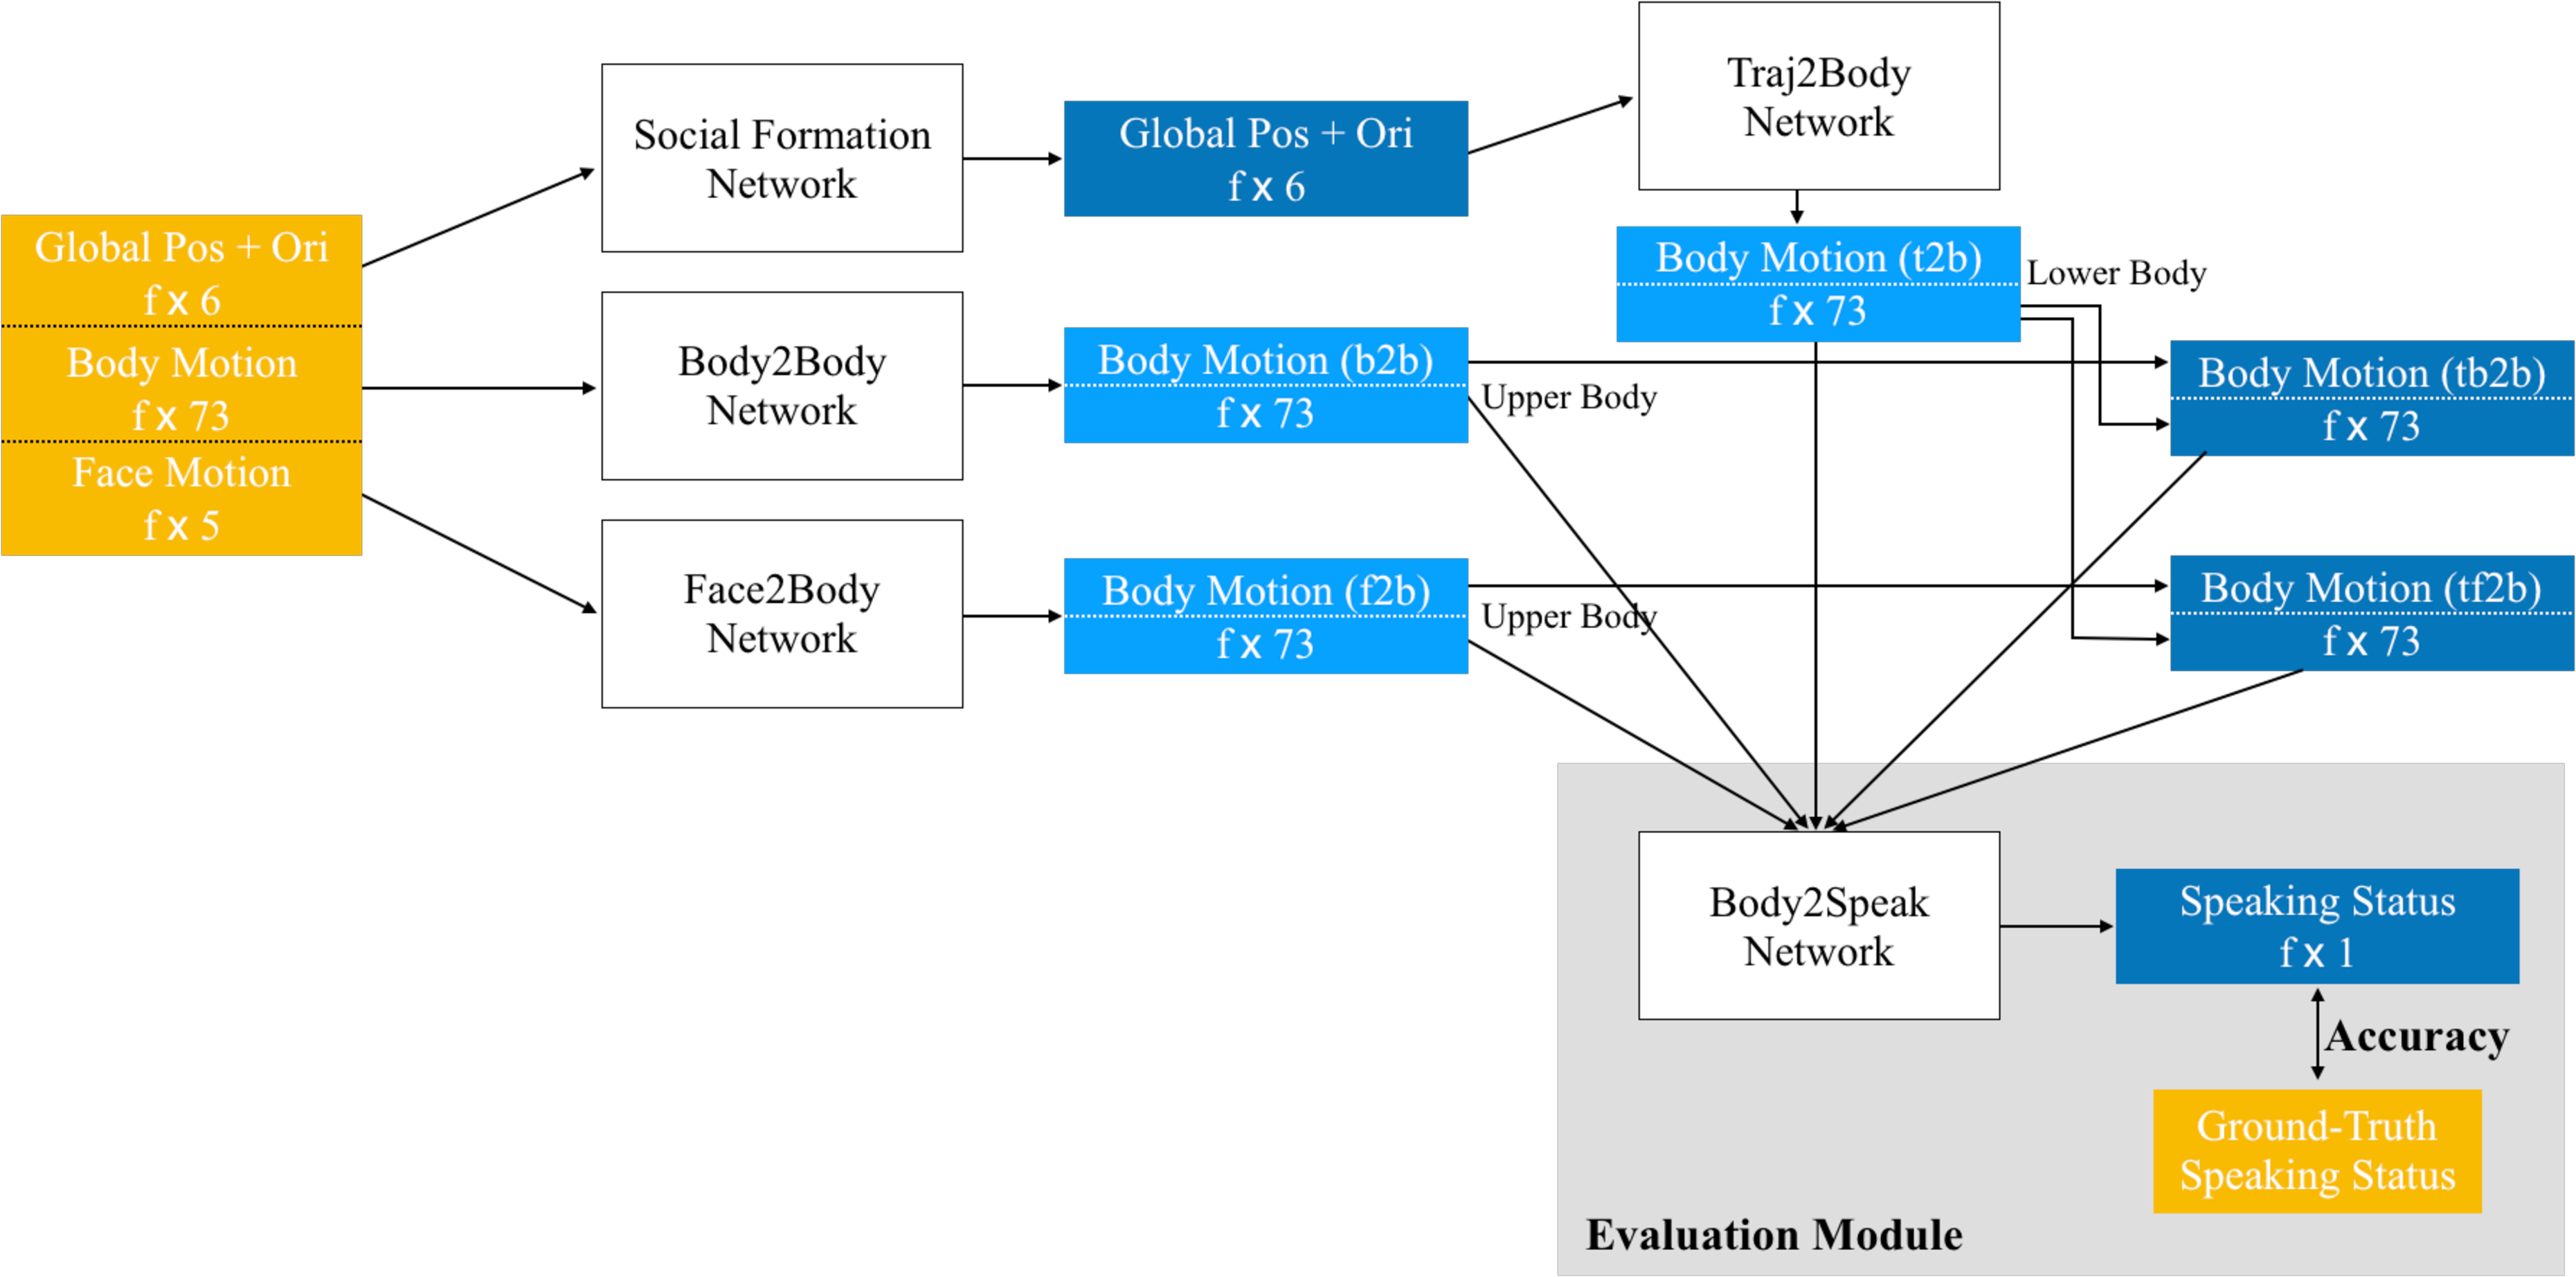
\includegraphics[ width=0.8\linewidth]{ssp_fig/evaluation_pipeline.pdf}
%%	\caption{Evaluating body motion prediction by speaking classification} 
%%	\label{fig:evaluation_bySpeakclass}
%%\end{figure}
%
%
%%The final outputs predict more natural social behaviors than other baselines, satisfying most of the noticeable social rules in the scenes (distance, orientation, leg and root movement, and natural hand motions). Our results are best seen in the supplementary videos. However, the quantitative errors tend to be higher, as shown in Table~\ref{table:predBody_errors} and Figure~\ref{chapter:predBody_errors}. Notably, the average pose computed from the training set shows the best performance. This is because the error metric computing the 3D errors from the ground-truth cannot fully evaluate how natural the motion appears. %Given the similar social signal inputs, there are diverse possible suitable human motions, and a better evaluation method is required to consider this.%  the quality of social signal prediction.% and it should be related to a 
%
%% {\color{red} Qualitative example where turn taking is captured?}
%
%% \noindent \textbf{Direct Regression from Social Formations:}
%% We can directly regress from the predicted 2D formation output.  
%
%% PCK curves 
%% Per joint
%
%
%% \textbf{Regression from Richer Input:}
%% We use other skeletons and input and see any improvement. 
%
%% Compared to the direct regression. 
%% {\color{red} Any semantic improvement which is not captured by numbers?}
%
%% Any good way to evaluate realistic human motion???
%
%
%% \subsection{Quantifying Social Signal Importance}